\setcounter{chapter}{5}
\chapter{Onde elettromagnetiche}

\section{Equazioni di Maxwell nel vuoto}

Il campo elettrico $\bold{E}(\bold{r},t) $ e il campo magnetico $\bold{B}(\bold{r},t)$ esistono quando sono presenti condizioni non stazionarie per la densit\`a di carica libera  $\rho(\bold{r},t)$ e la densit\`a di corrente libera $\bold{J}(\bold{r},t)$. L'interazione tra le cariche \`e descritta dalla forza $\bold{F} = q(\bold{E} + \bold{v} \times \bold{B})$ e le equazioni di Maxwell nel vuoto descrivono la relazione tra i campi  e le sorgenti:
\begin{align}
	& \nabla \cdot \bold{E} = \frac{\rho}{\varepsilon_0} \quad \text{Legge di Gauss} \\ \rule{0pt}{20pt}
	&\nabla \times \bold{E} = - \frac{\partial \bold{B}}{\partial t} \quad \text{Legge di Faraday} \\ \rule{0pt}{20pt}
	& \nabla \cdot \bold{B} = 0 \\ \rule{0pt}{20pt}
	& \nabla \times \bold{B} = \mu_0 \bold{J} + \varepsilon_0 \mu_0 \frac{\partial \bold{E}}{\partial t} \quad \text{Legge di Amp\`ere-Maxxwell}
\end{align}
Nel limite statico le soluzioni per $\bold{E}$ e $\bold{B}$ sono indipendenti, infatti le equazioni di Maxxwell assumono la forma 
\begin{equation*}
\left \{ \begin{array}{l}
	 \nabla \cdot \bold{E} = \frac{\rho}{\varepsilon_0}  \quad \quad  \nabla \cdot \bold{B} = 0 \\ \rule{0pt}{20pt}
	 \nabla \times \bold{E} = 0 \quad \quad  \nabla \times \bold{B} = \mu_0 \bold{J}\\ 
	\end{array}\right.
\end{equation*}
Nel limite quasi statico, il campo elettrico variabile dipende da $\bold{B}$, ma non il viceversa. Le soluzioni risultano dunque essere pi\`u complesse rispetto al caso statico perch\`e si hanno campo elettrico e campo magnetico accoppiati dalla legge di Faraday e dalla leggi di Ampere-Maxxwell.

Dallo studio di alcune configurazioni idealizzante, la cui relazioni tra campi e sorgenti \`e di facile deduzione, emergono delle propriet\`a principali della soluzione delle equazioni di Maxwell: 
\begin{itemize}
	\item \textit{principio di casualit\`a }: sorgenti variabili generano una perturbazione del campo magnetico che si propaga nel vuoto con velocit\`a $c$ pari a quella della luce. Poich\`e l'informazione si propaga con una velocit\`a finita $c$, il campo osservabile ad una certa distanza dalla sorgente \`e un campo che riflette ci\`o che \`e avvenuto alla sorgente ad un tempo precedente.
	\begin{equation*}
		\bold{E}(\bold{r},t) = \bold{E}\left(t - \frac{|r|}{c}\right) \quad \quad \bold{B}(\bold{r},t) = \bold{B} \left(t - \frac{|r|}{c}\right)
	\end{equation*}
	\item per le leggi sul flusso di $\bold{E}$ e $\bold{B}$, la perturbazione del campo \`e ortogonale alla direzione di propagazione. 
	\item per le leggi di Faraday e Amp\`ere-Maxxwell, il campo elettrico e magnetico variabili si autosostengono, sono mutualmente ortogonali, e hanno ampiezza legate dalla relazione 
	\begin{equation*}
		B = \frac{1}{c}E
	\end{equation*}
	\item la velocit\`a di propagazione della perturbazione \`e  
	\begin{equation*}
		c = \frac{1}{\sqrt{\varepsilon_0 \mu_0}}
	\end{equation*}
\end{itemize}

\subsection{Soluzioni ondulatorie delle equazioni di Maxxwell nel vuoto e all'esterno delle sorgenti}

La derivazione formale della propagazione per onde dei campi elettromagnetici nel vuoto la si ottiene scrivendo le equazioni di Maxxwell in regioni prive di sorgenti, $\rho(\bold{r},t) = 0$ e $\bold{J}(\bold{r},t) = 0$
\begin{equation*}
\left \{ \begin{array}{l}
	 \nabla \cdot \bold{E} = 0  \quad \quad \quad \quad   \nabla \cdot \bold{B} = 0 \\ \rule{0pt}{20pt}
	 \nabla \times \bold{E} = - \frac{\partial \bold{B}}{\partial t} \quad \quad  \nabla \times \bold{B} = \varepsilon_0 \mu_0 \frac{\partial \bold{E}}{\partial t}\\ 
	\end{array}\right.
\end{equation*}
Per disaccoppiare le equazioni applichiamo l'operazione di rotore ad entrambi i membri della legge di Faraday e di Amp\`ere-Maxxwell, e utilizziamo l'identit\`a vettoriale 
\begin{equation*}
	\nabla \times (\nabla \times \bold{A} ) = - \nabla ^2\bold{A} + \nabla (\nabla \cdot \bold{A})
\end{equation*}

Sostituendo $\bold{A} = \bold{E}$ si ha che 
\begin{equation*}
	\nabla \times (\nabla \times \bold{E}) = - \nabla^2 \bold{E} + \nabla (\underbrace{\nabla \cdot \bold{E}}_{=0}) = - \frac{\partial }{\partial t}(\nabla \times \bold{B})
\end{equation*}
restandoci l'equazione
\begin{equation}
	\nabla^2 \bold{E} = \varepsilon_0 \mu_o\frac{\partial^2 \bold{E}}{\partial t^2}
\end{equation}
analogamente ponendo $\bold{A} = \bold{B}$ si ha l'equazione:
\begin{equation}
	\nabla^2 \bold{B} = \varepsilon_0 \mu_0 \frac{\partial^2 \bold{B}}{\partial t^2}
\end{equation}
che hanno la stessa struttura dell'equazione delle onde di D'Alambert:
\begin{equation*}
	\nabla^2f = \frac{1}{c^2} \frac{\partial ^2f}{\partial t^2}
\end{equation*}
Le equazioni di Maxxwell in vuoto e in regioni prive di sorgenti hanno soluzioni ondulatorie. Confrontando le equazioni (6.6) e (6.5) con l'equazione di D'Alambert scopiamo che le onde elettromagnetiche nel vuoto si propagano alla velocit\`a 
\begin{equation*}
	c = \frac{1}{\sqrt{\varepsilon_0 \mu_0}}
\end{equation*}
Le misure sperimentali della velocit\`a della luce e di $1/\sqrt{\varepsilon_0 \mu_0}$ ci dicono che la luce \`e radiazione elettromagnetica.
\begin{remark}
\
\begin{itemize}
	\item Le equazioni (6.5) e (6.6)  ammettono soluzioni anche per campi che non soddisfano le equazioni di Maxxwell, tali soluzioni non possono descrivere campi elettromagnetici reali.
	\item Le equazioni (6.5) e (6.6) sono soddisfatte anche da campi uniformi e costanti, tali campi non hanno le caratteristiche di un'onda.
\end{itemize}	
\end{remark}
\section{Tipi di onda piana  soluzione dell'equazione di D'Alambert}
\subsection{Onde piane}
\begin{wrapfigure}{r}{0.5\textwidth}  % 'r' for right, 'l' for left
  \centering
  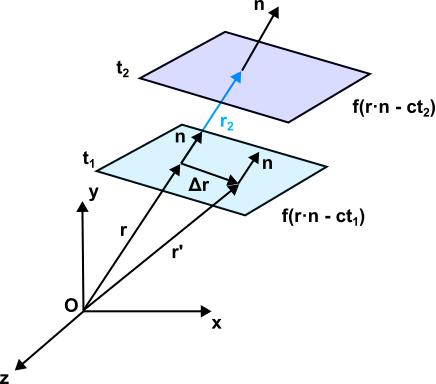
\includegraphics[width=0.49\textwidth]{images/planar_wave}
\end{wrapfigure}
Una delle soluzioni dell'equazione di D'Alambert tridimensionale \`e data da un'onda piana scalare, ed \`e rappresentata da una funzione
\begin{equation}
	f = f(\bold{r} \cdot \hat{n} \;\mp \; ct)
\end{equation}
dove il vettore
\begin{equation*}
	\bold{r} = x \hat{u}_{x} + y \hat{u}_{y} + z \hat{u}_{z}
\end{equation*}
\`e il raggio vettore che individua un punto nello spazio in un riferimento cartesiano, $\hat{n}$ \`e il versore che individua la direzione di propagazione dell'onda e $c$ \`e la velocit\`a con cui questa si propaga. Il prodotto vettoriale $\bold{r} \cdot \hat{n}$ \`e la proiezione della posizione del punto lungo la direzione di propagazione dell'onda.

La funzione f \`e definita in tutto lo spazio-tempo ed assume lo stesso valore (fronte d'onda) in tutti i punti in ci il suo argomento $\xi = \bold{r} \cdot \hat{n}  \; \mp \; ct$ (detta fase), ha lo stesso valore. Per ogni istante fissato, il luogo dei punti in cui f ha  un determinazione valore \`e un piano ortogonale alla direzione di propagazione dell'onda. Per dimostrarlo, osserviamo che 
\begin{equation*}
	f(\xi) = f(\xi') \quad \iff \quad \xi = \xi'
\end{equation*}
ad un istante $t$ fissato. Questo vuol dire che 
\begin{equation*}
	\bold{r} \cdot \hat{n} \pm ct = \bold{r}' \cdot \hat{n} \pm ct \quad \iff \quad (\bold{r}-\bold{r}') \cdot \hat{n} = 0 
\end{equation*}
questo vuol dire che $\Delta \bold{r}$ \`e appartiene ad un piano ortogonale alla direzione $\hat{n}$. 

Il fatto che l'onda piana si propaghi con una velocit\`a c lo si dimostra dal fatto che 
\begin{equation*}
	f(\xi_{1}) = f(\xi_{2}) \quad \iff \quad \xi_{1} = \xi_{2} 
\end{equation*}
questo equivale a chiedere che 
\begin{equation*}
	\bold{r}_{1} \cdot \hat{n} \pm ct_{1} = \bold{r}_{2} \cdot \hat{n} \pm ct_{2} \quad \iff \quad \Delta \bold{r} \cdot \hat{n} = \pm c(t_{2}-t_{1}) \quad \iff \quad \frac{\Delta \bold{r}}{\Delta t} \cdot \hat{n} =  \pm c
\end{equation*}
dimostrando che i piani in cui f \`e costante si propagano lungo la direzione $\hat{n}$ con velocit\`a $\pm c $ per onde progressive e regressive. In alternativa si pu\`o calcolare la veloicit\`a con cui si propaga il fronte d'onda d'onda imponendo: 
\begin{equation*}
	\frac{d \xi }{dt} = 0 \quad \Rightarrow \quad \frac{d \bold{r}}{dt} = \pm c
\end{equation*}
e prede il nome di \textbf{velocit\`a di fase}.

A questo punto non ci resta da dimostra per sostituzione come l'equazione (6.7) sia soluzione dell'equazione di D'Alambert tridimensionale:
\begin{equation*}
	\nabla^2 f(\bold{r} \cdot \hat{n} \mp ct) =\frac{1}{c^2}\frac{\partial^2 f(\bold{r} \cdot \hat{n} \mp ct)}{\partial t^2} 
\end{equation*}
mostrando come il termine di sinistra sia uguale a quello di destra e viceversa.

In generale in coordinate cartesiane abbiamo che per ciascuna componente:
\begin{equation*}
	\frac{\partial f}{\partial x} = \frac{\partial f}{\partial \xi} \frac{\partial \xi}{\partial x}
\end{equation*}
siccome $\xi = xn_{x} + yn_{y} + zn_{z} \mp ct $ si ha che ciascuna derivata \`e della forma:
\begin{equation*}
	\left \{ \begin{array}{l}
		\frac{\partial f}{\partial x} = n_{x} \frac{\partial f}{\partial \xi} \\ \rule{0pt}{20pt}
		\frac{\partial f}{\partial y} = n_{y} \frac{\partial f}{\partial \xi} \\ \rule{0pt}{20pt}
		\frac{\partial f}{\partial z} = n_{z} \frac{\partial f}{\partial \xi}
	\end{array}\right.
\end{equation*}
possiamo esprimere dunque l'operatore
\begin{equation*}
	\nabla = (n_{x} \hat{u}_{x} + n_{y} \hat{u}_{y} + n_{z} \hat{u}_{z}) \frac{\partial }{\partial \xi} = \hat{n} \frac{\partial }{\partial \xi} 
\end{equation*}
e quindi
\begin{equation*}
	\nabla^2 = \nabla \cdot \nabla = \hat{n} \frac{\partial }{\partial \xi} \cdot \hat{n} \frac{\partial }{\partial \xi} = \frac{\partial^2}{\partial \xi^2}
\end{equation*}
analogamente la derivata temporale pu\`o essere scritta come
\begin{equation*}
	\frac{\partial f}{\partial t} = \frac{\partial f }{\partial \xi} \frac{\partial \xi}{\partial t} = \mp c \frac{\partial f}{\partial \xi}
\end{equation*}
se deriviamo rispetto al tempo una seconda volta otteniamo
\begin{equation*}
	\frac{\partial^2 f }{\partial t^2} = c^2 \frac{\partial ^2f}{\partial \xi ^2}
\end{equation*}
e quindi i termini sia di destra che di sinistra coincidono.

\section{Onde piane monocromatiche}

Un onda piana monocromatica (o armonica) \`e un onda che risulta essere in funzione di una sola frequenza $\nu$ e la funzione f risulta avere graficamente un andamento sinusoidale.  Prima di darne una definizione analitica introduciamo un vocabolario che si una nella trattazione delle onde:
\begin{itemize}
	\item Definiamo \textbf{lunghezza l'onda (periodo spaziale)} $\bm{\lambda} \;\bold{[nm]}$ una grandezza fisica che rappresenta la \textbf{distanza tra due creste successive (o due punti equivalenti)} di un'onda periodica. \`E una grandezza a cui facciamo riferimento quando consideriamo lo sviluppo dell'onda nello spazio.
	\item Definiamo \textbf{periodo (T) [s]} il tempo impiegato da un'onda per compiere \textbf{un'oscillazione completa}, cio\`e ripetere una volta il suo ciclo. \`E una grandezza che viene utilizzata quando consideriamo lo sviluppo dell'onda nel tempo.
\end{itemize} 
Ritornando alla definizione di onda piana monocromatica questa da un punto di vista analitico viene espressa come:
\begin{equation}
	f(\bold{r},t) = A \cos(\bold{k} \cdot \bold{r} - \omega t + \phi)
\end{equation}
i parametri che compaiono nell'equazione hanno il seguente significato:
\begin{itemize}
	\item $\phi$ \`e il termine di fase iniziale dell'onda, legata all'ampiezza nell'origine $f(\bm{0},0)=A\cos \phi$;
	\item $\omega  =2 \pi /T$ \`e la frequenza angolare associata al periodo temporale T dell'onda (e alla frequenza $\nu = 1/T$);
	\item $\bold{k} = k \hat{n}$ \`e il vettore d'onda ( il modulo prende il nome di numero d'onda), parallelo alla direzione di propagazione dell'onda, con modulo $k = 2\pi / \lambda$ associato al periodo spaziale $\lambda$ (\textit{lunghezza d'onda}).
\end{itemize}
L'argomento del coseno dell'espressione (6.8) prende il nome di \textbf{fase totale dell'onda} $\xi$. La \textbf{velocit\`a} di fase per le onde monocromatiche \`e data dalla relazione:
\begin{align*}
	\frac{d \xi}{dt} = 0 \quad & \iff \quad \bold{k} \cdot \frac{d \bold{r}}{dt} - \omega = 0 \\ \rule{0pt}{20pt}
	& \iff \quad k \hat{n} \cdot \frac{d \bold{r}}{dt} - \omega = 0 \\ \rule{0pt}{20pt}
	& \iff \quad \hat{n} \cdot \frac{d \bold{r}}{dt} = \frac{\omega}{k} \\ \rule{0pt}{20pt}
	& \iff \quad v_{f} = \frac{\omega}{k} = \lambda \nu
\end{align*} 
Per ogni tipo di onda monocromatica esiste una relazione tra $\omega$ e $\bold{k}$, detta \textit{relazione di dispersione}. Questa relazione \`e dovuto alla struttura della fase totale dell'onda come si osserva dai passaggi per dedurre la velocit\`a di fase:
\begin{equation*}
	\omega (\bold{k}) = kv_{f}
\end{equation*}
Siccome l'onda \`e monocromatica il rapporto $\omega/k$ \`e costante, coincidendo con $v_f$ questo rappresenta la velocit\`a con cui si muovono i piani di egual fase, o \textbf{superfici d'onda} perprendicolari a $\hat{n}$.

Per le onde elettromagnetiche in vuoto la velocit\`a di fase \`e indipendente dalla frequenza.  Le onde devono soddisfare un'equazione delle onde, dedotta dalle equazioni di Maxxwell, ove compara la velocit\`a
\begin{equation*}
	c(k) = \frac{1}{\sqrt{\varepsilon_0}\mu_0}
\end{equation*}
Ne consegue che le componenti armoniche di una qualunque onda periodica reale si propagano nel vuoto alla stessa velocit\`a di fase e l'onda mantiene la stessa forma.

\subsection{Rappresentazione complessa di un'onda}
L'equazione (6.8) che rappresenta un onda monocromatica piana, pu\`o essere considerata come parte reale di una funzione complessa:
\begin{equation*}
	f = A\cos(\bold{k} \cdot \bold{r} \mp \omega t  + \phi) = \mathcal{R}e[Ae^{i(\bold{k} \cdot \bold{r} \mp \omega t + \phi)}]
\end{equation*}
dove possiamo raccogliere il termine $e^{i\phi}$ che prende il nome di termine di fase, questo vuol dire che le onde possono essere rappresentate in generale a meno di una fase. Tale relazione risulta essere comoda per trattare la sovrapposizione di pi\`u onde. 

Infatti le onde rigorosamente monocromatiche in natura non esistono e in realt\`a \`e utile la loro sovrapposizione che permette di dare una descrizione matematica pi\`u aderente alla realt\`a sperimentale. Questa descrizione \`e resa possibile grazie alla natura lineare dell'equazione delle onde e il teorema di Fourier. La rappresentazione complessa di un onda reale \`e data dall'espressione 
\begin{equation*}
	f(\bold{r},t) = \mathcal{R} \left[ \int_{- \infty}^{+ \infty} A(k)e^{i(\bold{k} \cdot \bold{r} \mp \omega t )}dk\right]
\end{equation*} 
dove l'integrale si estende su numeri d'onda positivi e negativi, che corrispondo rispettivamente a onde progressive e regressive.

\section{Campi elettromagnetici nelle onde piane}
\subsection{Onda piana uniforme (rappresentazione vettoriale)}

Abbiamo visto come le equazione di Maxwell per il campo elettrico e magnetico diano origine a equazione differenziale parziale del secondo ordine la cui struttura coincide con quella dell'equazione di D'Alambert. Data la struttura analoga le onde piane viste nella sezione precedente risultano essere soluzione dell'equazione dei campi, la domanda che dobbiamo porci \`e: " sotto quali condizioni soddisfano l'equazione dei campi ? "

Rappresentiamo il campo elettrico soluzione come un onda piana uniforme:
\begin{equation}
	\bold{E}(\bold{r},t) = \bold{E}_0 f(\bold{r} \cdot \hat{n} \pm ct)
\end{equation} 
dove c \`e la velocit\`a di fase di un'onda elettromagnetica che si propaga nel vuoto e la sua grandezza coincide con la velocit\`a della luce.

Una soluzione di questo tipo deve soddisfare le equazione di Maxwell, in assenza di sorgenti, le uniche che mancano da verificare sono:
\begin{equation*}
	\nabla \cdot \bold{E} = 0 \quad \quad \nabla \cdot \bold{B} = 0
\end{equation*}
Considerando le soluzioni per il campo elettrico, sostituendo l'espressione del campo otteniamo la condizione:
\begin{equation*}
	\hat{n} \cdot \frac{\partial \bold{E}}{\partial \xi} = 0
\end{equation*}
Poich\`e la direzione di propagazione dell'onda $\hat{n}$ \`e costante (in realt\`a \`e sufficiente che sia localmente costante), possiamo scrivere:
\begin{equation*}
	\frac{\partial}{\partial \xi}(\hat{n} \cdot \bold{E}) = 0
\end{equation*}
e dunque la componente parallela alla direzione di propagazione dell'onda $\bold{E}_{\hat{n}} $ \`e costante. Questo vuol dire che il campo elettrico variabile pu\`o esiste solo nel piano ortogonale ad $\hat{n}$. Inoltre la natura di questo campo \`e associato a sorgenti di natura statica.

Le medesime condizioni e quanto discusso vale in maniera analoga per il campo magnetico $\bold{B}$.

\subsection{Relazioni tra campo elettrico e magnetico}

Assumiamo di avere campo elettrico e campo magnetico per cui vale la seguente condizione:
\begin{equation*}
	\bold{E} \cdot \hat{n} = \bold{B} \cdot \hat{n} = 0
\end{equation*}
possiamo tranquillamente assumere questa condizione, perch\`e tanto il campo nella direzione di propagazione \`e una costante e per comodit\`a di conto scegliere che questo sia nullo. In questo modo deriviamo la prima propriet\`a che lega $\bold{E}$ e $\bold{B}$:

\begin{center}
\fbox{\parbox{15cm}{ Per un onda elettromagnetica piana che si propaga liberamente nel vuoto i campi $\bold{E}$ e $\bold{B}$ sono ortogonali alla direzione di propagazione. Quindi i due campi si propagano nello stesso verso.}}
\end{center}
Dalla legge di Amp\`ere-Maxxwell abbiamo che le soluzione del  campo elettrico e del campo magnetico sono legate tra loro:

\begin{equation*}
	\nabla \times \bold{E} = - \frac{\partial \bold{B}}{\partial t}
\end{equation*}
dato che possiamo esprimere l'operatore nabla come:
\begin{equation*}
	\nabla = \hat{n} \frac{\partial }{\partial \xi}
\end{equation*}
l'equazione di A-M diventa:
\begin{align*}
	\hat{n} \frac{\partial}{\partial \xi} \times \bold{E} = - \frac{\partial \bold{B}}{\partial t} \quad & \iff \quad \frac{\partial}{\partial \xi}(\hat{n} \times \bold{E}) = - \frac{\partial \bold{B}}{\partial \xi} \frac{\partial \xi}{\partial t} \\ \rule{0pt}{30pt}
	& \iff \quad \frac{\partial}{\partial \xi}(\hat{n} \times \bold{E}) = \pm c \frac{\partial \bold{B}}{\partial \xi} \\ \rule{0pt}{30pt}
	& \quad \Rightarrow \quad \hat{n} \times \bold{E} = \pm c\,\bold{B}
\end{align*}
da cui otteniamo la relazione compatta:
\begin{equation}
	\bold{B} = \frac{\pm \hat{n} \times \bold{E}}{c} = \frac{\bold{c} \times \bold{E}}{c^2}
\end{equation}
tale relazione ci dimostra due importanti risultati:

\begin{center}
	\fbox{\parbox{15cm}{Per un onda elettromagnetica che si propaga nel vuoto liberamente i campi $\bold{E}$ e $\bold{B}$ sono \textbf{mutualmente ortogonali} tra loro e il loro rapporto \`e pari alla velocit\`a della luce $B/E =c$}}
\end{center}
Le direzioni (orientate) di $\bold{E}$, $\bold{B}$ e della velocit\`a di fase $\bold{c}$ rappresentano nell'ordine indicato ($\bold{E},\bold{B},\bold{c}$) una terna destrorsa, sia per le onde progressive che per le onde regressive.

\begin{center}
	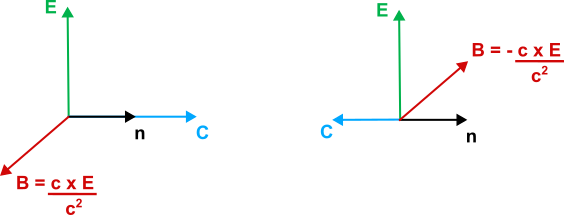
\includegraphics[width = 11cm]{images/nxe}
\end{center} 

\subsection{Polarizzazione lineare}

La relazione (6.10) fisse le direzioni relative del campo elettrico e del campo magnetico , solo in termini locali. In generale il campo elettrico (e di conseguenza anche quello magnetico) non mantiene sempre la stessa direzione nel tempo. Il comportamento del campo dipende dalla natura della sorgente. Se il campo elettrico mantiene nel tempo sempre la stessa direzione, l'onda si dice \textbf{polarizzata linearmente} lungo tale direzione.

Nel caso di un onda sinusoidale, linearmente polarizzata il campo \`e della forma nella seguente figura.
\begin{center}
	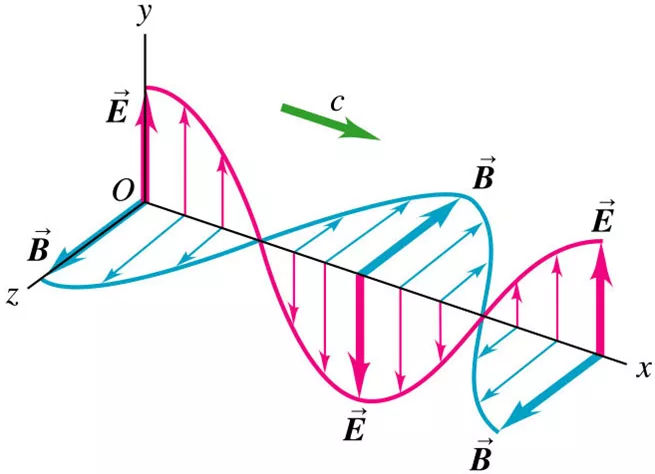
\includegraphics[width = 9cm]{images/linear_pol}
\end{center}

\section{Tipi di onda sferica soluzione dell'equzione di D'Alambert }

\subsection{Onde sferiche }

Tra le funzione soluzione dell'equazione delle onde di D'Alambert troviamo quelle che vengono definite onde sferiche, ovvero funzioni d'onda dipendenti solo dal tempo e dalla distanza radiale $\bold{r}$ dalla sorgente che si propagano con velocit\`a $c$:
\begin{equation}
	\psi(\bold{r},t) 
\end{equation}
Le onde sferiche sono associabili a sorgenti di emissione localizzate nello spazio. Inoltre risultano essere aprossimabili localmente ad onde piane, ovvero date pi\`u sorgenti sferiche se fatte collimare li linee di propagazione queste formano delle onde piane.

Verifichiamo che una funzione della forma (6.11) sia soluzione dell'equazione delle onde; per farlo ipotizziamo di avere una sorgente puntiforme in $\bold{r}(0,0,0)$ e che il sistema sia a simmetria sferica, dunque possiamo esprimere l'equazione di D'Alambert in coordinate sferiche:
\begin{equation}
	\nabla^2 \psi - \frac{1}{v^2} \frac{\partial^2 \psi }{\partial t^2} = 0
\end{equation}
dove l'operatore $\nabla^2$ assume l'espressione:
\begin{equation*}
	\nabla^2 \psi = \frac{1}{r}\frac{\partial}{\partial r^2}(r\psi)
\end{equation*}
di cui possiamo ignorare le componenti lungo $\phi$ e $\theta$ non essendoci dipendenza da parte di $\psi$. L'equazione (6.12) diventa:
\begin{equation*}
	\frac{1}{r}\frac{\partial^2}{\partial r^2}(r\psi) = \frac{1}{v^2} \frac{\partial^2 \psi }{\partial t^2}
\end{equation*}
e ammette soluzione solo nei punti $\bold{r} \neq \bm{0}$. Dato che $r$ non dipende dal tempo possiamo esprimere l'equazione precedente come:
\begin{equation*}
	\frac{\partial^2(r\psi)}{\partial r^2} = \frac{1}{v^2} \frac{\partial^2 (r\psi) }{\partial t^2}
\end{equation*}
questo ci dice che la funzione d'onda che soddisfa l'equazione deve essere della forma:
\begin{equation}
	f(\bold{r},t) = r \, \psi(\bold{r},t)
\end{equation}
Poich\`e anche funzioni d'onda $f(\bold{r} \mp vt)$ sono soluzioni ammesse dall'equazione (6.12) possiamo dedurre dalla funzione (6.13) che 
\begin{equation}
	\psi(\bold{r},t) = \frac{1}{r}f(\bold{r}\mp vt)
\end{equation}
dimostrando che $\psi$ ha proprio l'espressione che si era ipotizzata all'inizio.

La soluzione (6.14) rappresenta un'onda di forma fissa e ampiezza variabile in ragione del reciproco della distanza dall'origine. Le onde sferiche sono letteralmente superfici sferiche si propagano radialmente con velocit\`a v.
\begin{itemize}
\item Per convenzione anche se si ha sia una soluzione per un onda progressiva che per una regressiva, le onde sferiche le consideriamo solo progressive:
\begin{equation*}
	\psi(\bold{r},t) = \frac{1}{r}f(\bold{r}-vt) \quad \hat{n} = \hat{u}_{r}
\end{equation*}
\item Si pu\`o rendere esplicita la dipendenza dell'onda sferica dalla fase temporale $\zeta = (t-r/v)$, anzich\`e dalla fase spaziale, indicando con $g(t-r/v)$ la funzione composta $g(\zeta) = f(\xi(\zeta))$ dove $\xi = -v\zeta$. L'espressione dell'onda sferica assume la forma:
\begin{equation*}
	\psi(\bold{r},t) = \frac{1}{r}g(t-r/v)
\end{equation*}
Il termine $r/v$ mette in risalto il tardo associato alla velocit\`a finita di propagazione della perturbazione (cusalit\`a).
\item L'onda sferica \`e approssimabile a un'onda piana quando ci si trova a grande distanza dalla sorgente dove il raggio di curvatura \`e molto grande, e quando si guarda una porzione locale del fronte d'onda.
\item L'origine \`e un punto di singolarit\`a per la soluzione. Dunque si deve trovare una strategia per raccordare l'informazione della sorgente nella soluzione. Se eliminiamo la dipendenza del tempo l'equazione (6.12) diventa $\nabla^2 \psi = 0$ che corrisponde all'equazione di Laplace che si \`e vista nella trattazione dell'elettrostatica.
\begin{equation*}
	\frac{1}{r} \frac{\partial^2(r \psi)}{\partial r^2} = 0
\end{equation*}
Cercando soluzioni per $r \neq 0$, e fissando le costanti d'integrazione con le condizioni al contorno si ha:
\begin{equation*}
	\frac{d^2 (r \psi)}{d r^2} = 0 \quad \Rightarrow \quad r\psi = ar+b \quad \Rightarrow \quad \psi(r) = a + \frac{b}{r}
\end{equation*}
Posto $\psi(\infty) = 0 $ come condizione al contorno si ha $a = 0$. La costante $b$ \`e fissata dalla sorgente nell'origine del sistema.

\end{itemize}

\subsection{Campo elettromagnetico nelle onde sferiche}


